\testsection{Title-option}
\begin{tikzpicture}
\begin{loglogaxis}[title=A test title,xlabel=Dof,ylabel=Error]
\loglogtestplot
\end{loglogaxis}
\end{tikzpicture}

\testsection{Filter test}
{%
\def\myOwnYfilter#1\to#2{%
	\def#2{0.5}%
}%
\begin{tikzpicture}
\begin{axis}[yfilter={\myOwnYfilter}]
\addplot plot coordinates {
	(4,0)
	(6,1)
};
\end{axis}
\end{tikzpicture}
}%

\testsection{Test for addplot+[...]}
{
\tikzstyle{every axis legend}+=[at={(1.03,1)},anchor=north west]
\begin{enumerate}
	\item Ohne aenderung:

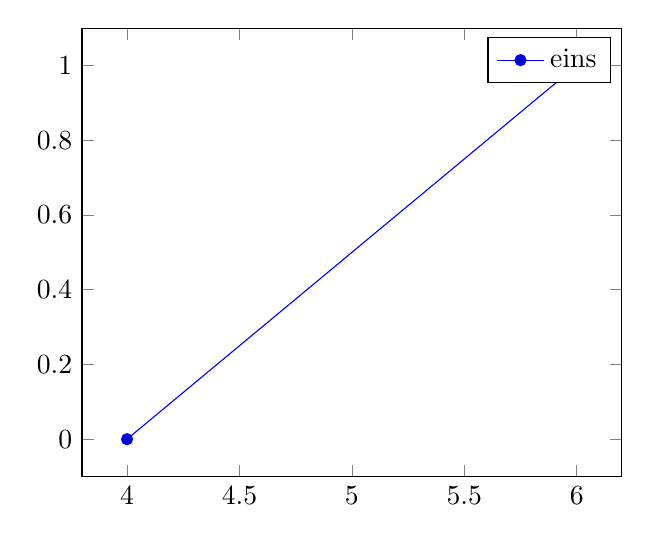
\begin{tikzpicture}
\begin{axis}
\smallplotstest

\addplot plot coordinates {
	(4,0)
	(6,1)
};
\legend{eins\\zwei\\}%
\end{axis}
\end{tikzpicture}

\item MIT aenderung:

\begin{tikzpicture}
\begin{axis}
\smallplotstest

\addplot+[only marks] plot coordinates {
	(4,0)
	(6,1)
};
\legend{eins\\zwei\\}%
\end{axis}
\end{tikzpicture}
\end{enumerate}
}

\testsection{Hide axis test}
\begin{tikzpicture}
	\begin{axis}
		\smallplotstest
	\end{axis}
\end{tikzpicture}
\begin{tikzpicture}
	\begin{axis}[hide axis]
		\smallplotstest
	\end{axis}
\end{tikzpicture}
\vskip 1cm
\noindent
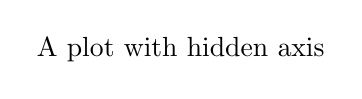
\begin{tikzpicture}
	\begin{axis}[hide axis,title=A plot with hidden axis]
		\smallplotstest
	\end{axis}
\end{tikzpicture}
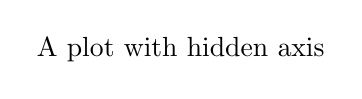
\begin{tikzpicture}
	\begin{axis}[hide axis,title=A plot with hidden axis]
		\smallplotstest
		\legend{A legend\\}
	\end{axis}
\end{tikzpicture}

